\chapter{Neural Network Classifier architecture}\label{chap5}

In the previous chapters, after a theoretical introduction of the concept of Artificial Neural Networks and of the type of task we are interested in solving, we show how to extrapolate and preprocess the information about the traffic data inside a network in order to train a classifier.

In this chapter we will propose a type of architecture able to solve this task, in \secref{modelprop}, and some  alternative classifier structures, obtained modifying the proposed one, in \secref{modelalt}. All the proposed classifier models, whose training results are presented in \chapref{chap6}, have been implemented inside the Keras framework and, in particular, using the Function API of this framework. 




\section{The proposed NN Classifier architecture}\label{modelprop}

In the previous chapter we described how each device, inside a device class, can be represented by a group of normalized time series and a vector of binary values. This double representation provides a lot of useful information to the classifier, but presents a challenge for its architecture. In common machine learning application in fact the ideal architecture, for the learning process over group of time series, would be a Convolutional Neural Network (CNN), described in \secref{cnn}, while, for a binary vector, the best performances are obtained using a Dense Neural Network (DNN), described in \secref{dnn}, composed of dense layers.
Even though it is possible to adapt one of the two architecture to learn using both representations as input, this choice would not exploit all the information that has been extract. 

The proposed architecture is then an "hybrid" model composed of both convolution and dense layers.
This model for the classifier architecture is shown in \figref{fig:1b_model}. As we can see the model presents two separate input layers, one for each representation. The time series input is then followed by a series of convolutional layers alternated with pooling layers, in order to reduce the input dimensionality. The communication protocol input, on the other hand, is forwarded to a single dense layer. On this dense layer the dropout technique is also implemented.

After the last convolutional layer the output of the convolutional branch is flattened, namely reduced to a one dimensional vector, and concatenated with the output of the dense layer from the communication protocol branch. The concatenated vector is then forwarded to four dense layers,  whose output at the end is the final prediction of the model. In the following sections we will analyze in depth each part of the proposed model alongside with the hyperparameters\footnote{The hyperparameters of a model are parameters left free during the creation of the model and are usually selected of specified when the model itself is instantiated but are fixed during its training. Example of hyperparameters are the number of neurons in a layer or the optimization algorithm to use.} of both the model architecture and training procedure.


\begin{figure}
    \centering
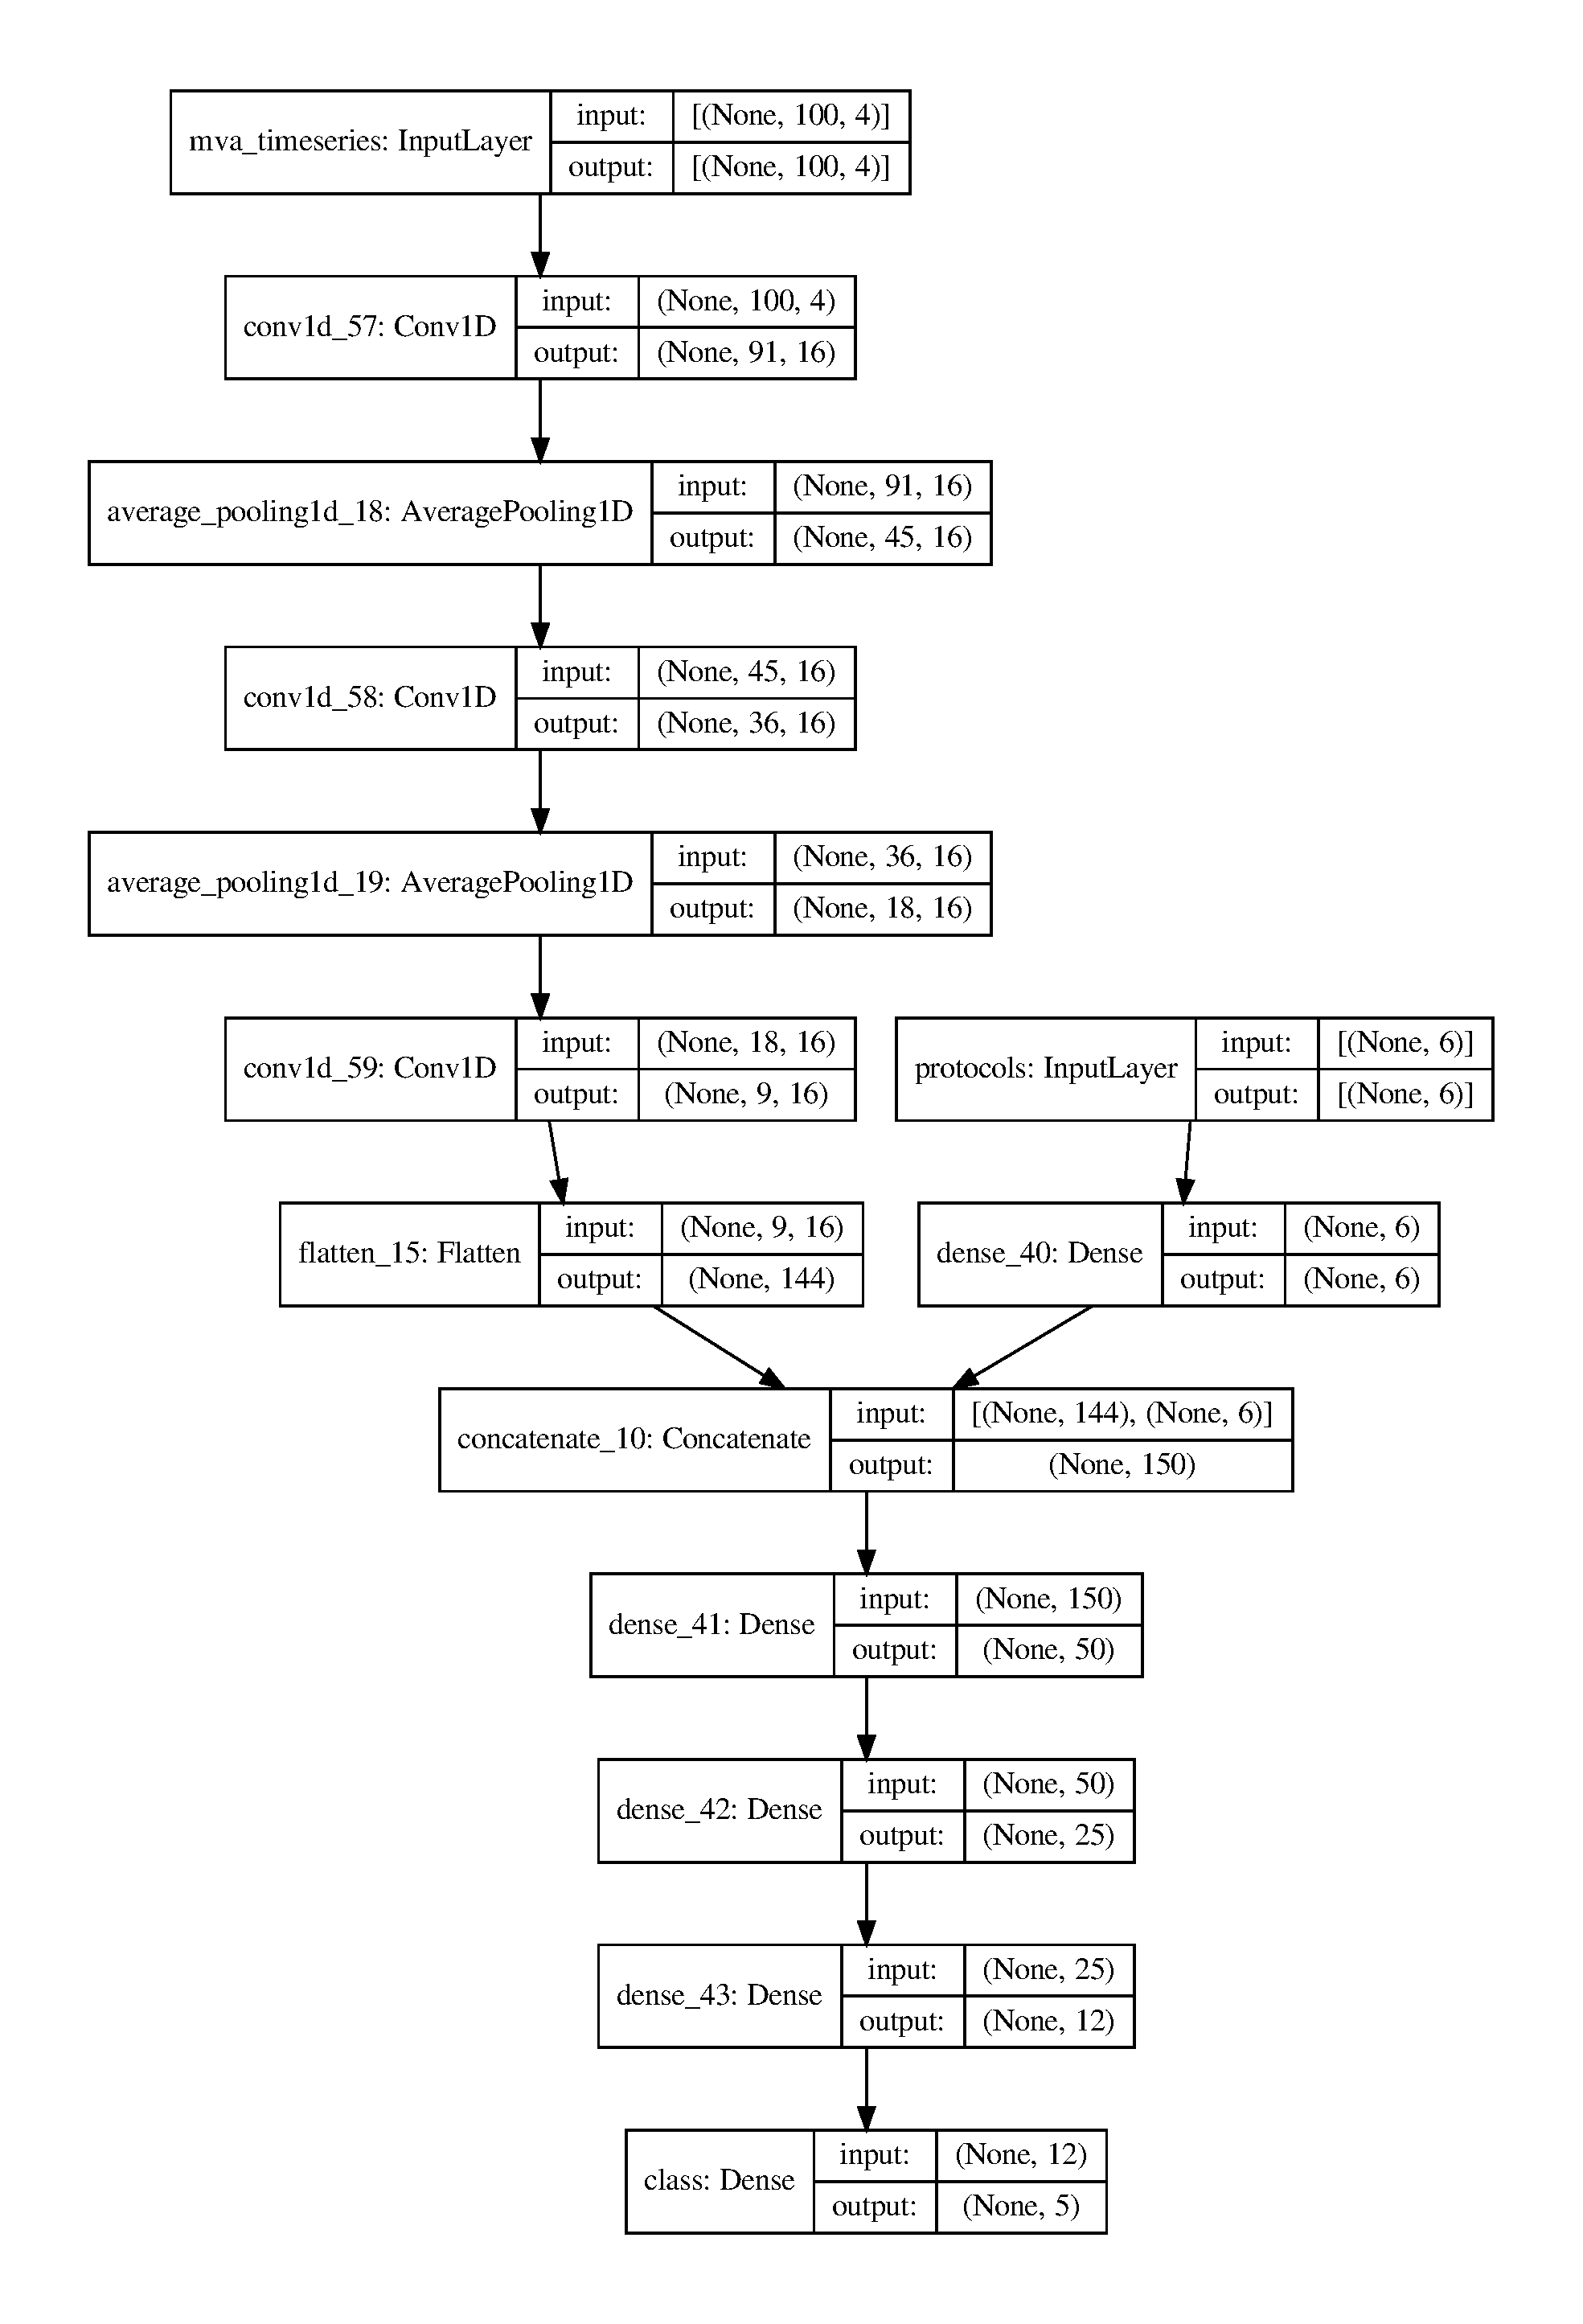
\includegraphics[height=0.95\textheight]{images/models/model_1bap.pdf}
\caption{{Structure of the proposed classifier 1B\_AP architecture. The name indicates the presence of only one convolutional branch and the use of average pooling layers.}}
    \label{fig:1b_model}
\end{figure}


\subsection{Time series analysis}

The convolution branch of the proposed model has the role of extracting information regarding the provided traffic time series. The choice of a convolutional architecture for this type of task has many advantages. In first place convolutional layers are the optimal choice due to their ability of of better understanding non-linear patterns with respect to a simple dense layers. Another great advantage is also the number of free parameters introduced by each layer, as we said in \secref{dnn}, the main drawback of a dense architecture is the high number of free parameters introduced by each layer. The use of convolutional layers therefore allows the creation of a deeper architecture while also containing the number of parameters.

In this architecture we use three convolutional layer, each one with the same number of filters and same filter size. The filter parameters can be selected as an hyperparameter at the creation of the model, in order to better adapt to the length of the input value. After each convolutional layer the ELU activation function, shown in \figref{fig:elu}, is applied to the output values before being passed to the following layers. An L2 regularization function, described in \secref{regularization}, is also introduced in each layer.

Between convolutional layers an average pooling layer is introduced. The pooling layers have the important role of reducing the dimensionality of the input values, with the goal of reducing the number of elements of the final output. This is important since the final prediction of the architecture is performed, as said before, using dense layers. An high dimensional input to the final layers will then translate in a very high number of parameters which may result in overfitting issues or in the inability of the model to be trained given the amount of samples in our dataset. The pool size of the average pooling layers is fixed to 2, namely the layers will return as output the average values of the input values taken in pairs.

\subsection{Communication protocol analysis}
The communication protocol input is processed using a dense layer. In this situation a dense layer is the optimal choice due to the reduced dimension of the input values, which allows to have a low number of free parameters. Recalling that each binary value of the input represent the eventual use of a class of protocols by the device, a dense layer has the advantage of being able to understand the importance of each single value and its relation with the others, respect to a convolutional layer which would search for patterns in the input.

As previosly said for this layer the dropout technique, described in \secref{dropout}, is introduced. The introduction of a dropout not only allows to avoid an eventual overfitting over the communication protocol input, possible in cases where many devices shares exactly the same protocol classes, but, more importantly, allows to regulate the importance of the communication protocol branch, with respect to the time series one. The value of the dropout rate does in fact regulate how many dense units are disconnected from the network, with the overall effect of reducing the importance of the output as the rate increases.
For this work the dropout was implemented using a dropout rate of 30\%.
As for the convolutional branch after the dense layer the ELU activation function is applied to the output and an L2 regularization in introduced.

\subsection{Final prediction}

After being separately processed, the information extrapolated by the model, from the two representation of the devices, must be combined to obtain a final prediction. 
In order to combine the output of the two branches the first step is to adapt the 2-dimensional output of the convolutional branch to the one dimensional output of the dense one. This operation is done using a flattening layer at the end of the convolutional branch, as the name suggests this layer converts the output matrix to a one dimensional vector by simply concatenating the values row-wise.
The combination of the two output is then performed using a concatenation layer which, as the name suggests, concatenates the two output to a single vector.

The resulting vector is then used a input for the last part of the classifier composed of four dense layers. The first three layers present an encoder structure, namely the number of neuron is halved in each layer, in order to reduce the dimensionality of the output values. The number of neurons of the first layer is left as an hyperparameter of the model. The number of neuron of the second and third layer is then fixed respectively as half and a forth of the number of neurons of the first one. Like for the previous layers also for these the ELU activation function is applied to the output of each layer and the L2 regularization is implemented in the computation of the loss function.

The last layer of the classifier model is again a dense layer but its structure must be adapted in order to produce the final prediction for the classification task. 
Since we are interested in solving a multiclass classification problem, we need as many output values as the number of classes of the task. This number is again left as an hyperparameter of the model and must be specified at the creation of the classifier. Each output values is then interpreted as the probability of sample to belong to a specific class. In order to interpret the output values as probabilities we also need to constrain the output values in the $[0;1]$ interval, which is done applying the Softmax\footnote{The softmax function maps a vector $\bar{z}\in \mathbb{R}^K$ to a probability distribution of K probabilities. This function is then a map $\sigma:\mathbb{R}\to[0,1]^K$ defined as:
\begin{equation}
\sigma(\mathbf{z})_{i}=\frac{e^{z_{i}}}{\sum_{j=1}^{K} e^{z_{j}}} \quad \quad i=1, \ldots, K \qquad\bar{z}=\left(z_{1}, \ldots, z_{K}\right) \in \mathbb{R}^{K}
\end{equation}} activation function to the output values.

If case of a binary classification, namely in case were interested in discriminating between only two classes, this last layer would instead be composed of a single neuron, with a Sigmoid activation function, shown in \figref{fig:act_sig}. The output would then be scalar value interpreted as the probability of belonging to the first class.

\subsection{Training hyperparameters}

Aside from the architecture hyperparameters, such as the number of neurons and filters in the various layers, some other hyperparameters must be specified before the start of the training procedure. 

The first hyperparameter to specify is the loss function to use in the estimation of the optimal model parameters. As we saw in \secref{lossfunction} many possible choices are possible. 
The suggested loss function, also implemented in this work, is the Categorical Cross Entropy,
which is a standard choice for the multiclass classification task. In case of binary classification we would instead suggest the use of the Binary Cross Entropy. Alongside this loss function we also use the L2 regularization, directly implemented in each layer, as described in the previous sections, in order to reduce the possibility of overfitting over the training set.

The second hyperparameter to choose is the optimization algorithm to use in order to minimize the loss function, during the application of the backpropagation algorithm. 
The chosen optimization algorithm is the Adam optimized, whose pseudo-code is shown in \algoref{alg:adam}.
This choice was mostly due to the "hybrid" structure of the network. Given the presence of both convolutional and dense layers, in two separated branches, the capability of the Adam algorithm of adapting the learning rate of each free parameters allows a faster convergence during the training procedure and often results in a more robust classifier.

The last hyperparameter to specify are the metrics to monitor during the training procedure, aside from the value of the loss function which is computed by default. Since we are interested in evaluating the ability of the model to perform a classification the accuracy metric, defined as the ratio between correct predictions over the total number of elements, has been selected. 

The choice of these three parameters is also known as model compilation, in the Keras framework. Once the model is compiled it is possible to start the training procedure, using the specified optimizer and loss, in order to obtain a trained classifier.

\section{Architecture variants} \label{modelalt}

In the previous sections we analyzed in depth the proposed architecture for a multiclass classifier, able to exploit both the time series and protocol communication input. This architecture is however not the only possible one. In the following sections we present some alternative architectures, obtained as a modification of the one presented before. These alternative architectures shares most features with the presented one but may result in a better performing classifier for different datasets. The model compilation and the hyperparameters are the same for all the possible arhcitectures. 
In order to better distinguish the possible alternatives we will refer to the original model as the 1B\_AP model.\footnote{This notation is used to indicate the number of branches and the pooling type of the model architecture. 1B stands for one convolutional branch, e.g. the original model, while 2B stands for two branches, namely models presented in \secref{2bmodels}. AP inidcates the use of average pooling layers between the convolutional ones, the alterantive is NP which indicates the absence of pooling layers, such as in the architecture presented in \secref{npmodels}.  }

\subsection{No pooling architecture}\label{npmodels}

The first proposed alternative architecture is, as we will see in the following chapter, the one used to create a classifier for the IoT Sentinel dataset, This architecture is designed for cases where the quantity of traffic captured is low. In this situations the lookback value $L$, introduced in the previous chapter, must be kept low in order to maximize the number of obtained samples, resulting however in shorter time series. 

If the dimensionality of the input array is already small, the pooling layers are then not only not necessary, but may even cause an issue where the number of output values is reduced to a point where the classifier is not able to use the extrapolated information in the following layers.
To solve this issue we propose an alternative architecture, shown in \figref{fig:1bnp_model}, where the pooling layers are removed and substituted with convolutional ones. The convolutional branch will then be composed of five consecutive convolutional layers.

Since this model is meant to be used in case of short time series the zero padding technique is also implemented in the convolutional layers. This technique consists in padding with zeros the start and the end of the input vector, before the application of the filters, in order to obtain an output vector with the same number of elements. Having a constant number of input and output values allows to avoid the risk, described before, of incurring in a too extreme reduction of the dimensionality and, consequently, in a bad performing classifier.
In the following we will refer to this architecture as the 1B\_NP model. 

\begin{figure}
    \centering
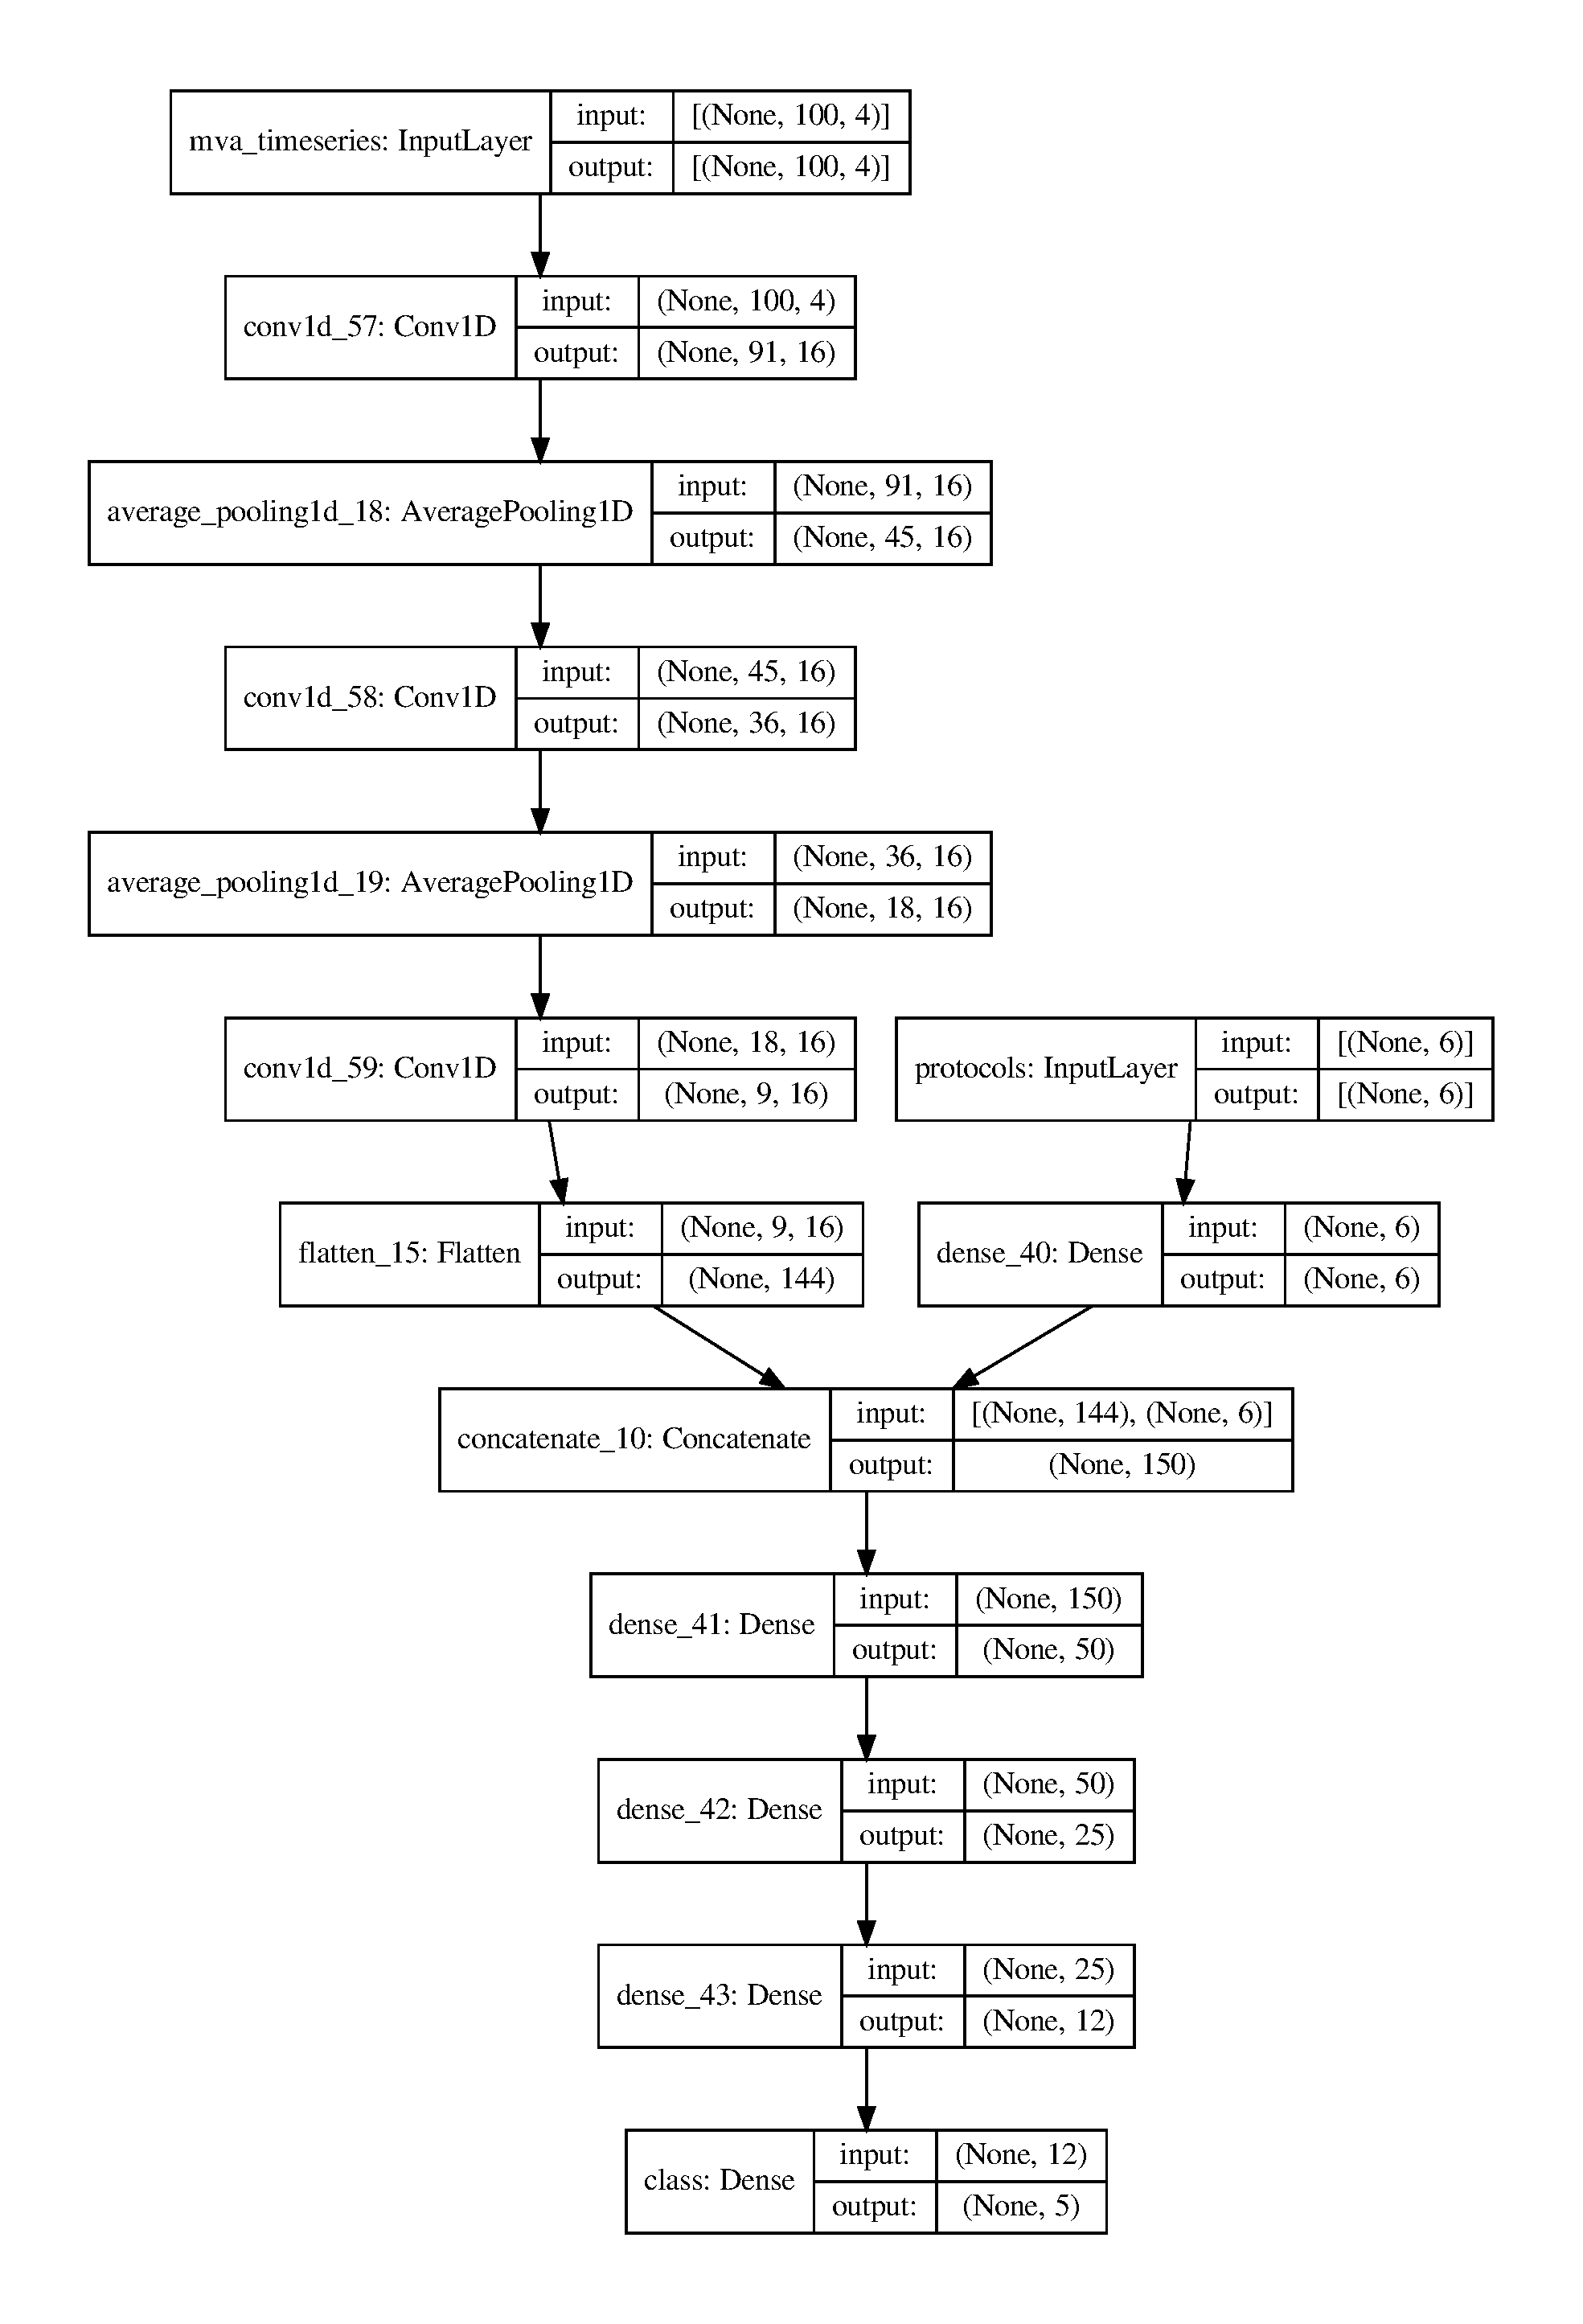
\includegraphics[height=0.95\textheight]{images/models/model_1bnp.pdf}
\caption{{Structure of the proposed classifier 1B\_NP architecture. The name indicates the presence of only one convolutional branch and the absence of pooling layers.}}    \label{fig:1bnp_model}
\end{figure}

\subsection{2 branches architecture}\label{2bmodels}

Another possible modification to the original structure is to separately process the time series containing the information regarding the transferred bytes and packets. This can be done introducing a splitting layer after the time series input layer which, as the name suggests, splits in two parts the received input. Each part of the input is then forwarded to a convolutional branch, with the same characteristics as the ones described for the previous architecture.

This architecture will then feature two convolutional branches with the possibility og them being either with average pooling layers (2B\_AP model in the following) or without pooling layers (2B\_NP model in the following). The advantage of this architecture is its capability of having a better performance in some specific binary classification cases but suffers from the main drawback of a really high number of free parameters. For this reason this architecture should be used for specific purposed classifications and not as a general approach to the device identification task. An example of the implementation of this architecture can be its use as a second level classification inside the device classes previously defined. 
In \appref{app:2bmodel} this type of architecture, both with and without pooling layers, is shown.

